% \chapter{Outils d'aide à la planification}
\section{Outils d'aide à la planification}

\subsection{Le contexte}%
\paragraph{}
La gestion de l'emploi du temps d'une équipe de 15 personnes ayant des rythmes différents peut être très problématique. C'est pourquoi, j'ai du réaliser un outils d'aide à la planification. Le but étant d'automatiser un maximum de tâches. 

On peut considérer deux rythmes différents minimum : le rythme des techniciens et le rythme des autres. Le rythme d'un technicien peut changer suivant la semaine et la période. En effet, un technicien peut travailler entre 8 et 10 heures par jour, mais il n'est pas forcé que tous les techniciens travail 7 heures ou 10 heures. Un roulement entre les techniciens peut se faire. 
Dans la suite du rapport on appellera une "plage horaire" un "rythme" correspondant à un ou plusieurs techniciens.
On considère aussi qu'une journée est composée de plusieurs plages horaires et qu'une semaine compte sept jours ouvrables de 8 heures à 23 heures.

\paragraph{}
On définit comme contrainte une limite que l’outil doit pendre en compte lorsqu'il génère un emploi du temps. Par exemple : un technicien doit avoir un weekend de deux jours consécutifs minimum par semaine. 
La première liste de contraintes à respecter est celle du Code du Travail. Cependant, au delà du code du travail, d'autres contraintes sont définies. Parmi elles ont peut cité par exemple : 
\begin{enumerate}
  \item Au moins 5 techniciens doivent être présent par jour
  \item Il ne doit pas y avoir de trous dans la journée d'un technicien
  \item 2 techniciens doivent commencer leur journée à 8 heures et 2 techniciens doivent terminer à 23 heures
\end{enumerate}
La gestion de l'emploi du temps est très problématique car les jours fériés et les dimanches sont travaillés et donc majorés. De plus certains techniciens ont des enfants à charge, ils ne peuvent donc pas avoir des horaires aussi flexibles que les autres.




\subsection{La réalisation}%
\paragraph{}
\newacronym{api}{API}{\foreignlanguage{english}{Application Programming Interface (Interface de programmation)}}
\newglossaryentry{apidef}{name={interface de programmation},description={Une interface de programmation est une façade clairement délimitée par laquelle un logiciel offre des services à d'autres logiciels. cf. \url{http://fr.wikipedia.org/wiki/Interface_de_programmation}}}

\newacronym{dom}{DOM}{\foreignlanguage{english}{Document Object Model}}
\newglossaryentry{domdef}{name={Document Object Model},description={Standard indépendant de tout langage de programmation permettant la modification de documents XML et HTML. cf. \url{http://fr.wikipedia.org/wiki/Document_Object_Model}}}
Afin de répondre au mieux aux attentes de l'équipe de techniciens et au maître d'apprentissage, j'ai demandé l'avis de quelques professeurs quant à la réalisation technique de cette outil. M.~Chan \textsc{Leduc} m'a suggéré un projet de fin d'année collant parfaitement avec ma mission en entreprise. Parmis les solutions techniques retenues, il y a Alloy(cf. figure~\ref{GUIalloy} page~\pageref{GUIalloy}), un langage déclaratif qui permet de mettre en place simplement un modèle représentatif d'un emploi du temps. 
Afin d'illustrer mon propos, l'image~\ref{solution} page~\pageref{solution} représente la solution (avant d'être interpréter) issue du modèle Alloy de mon entreprise.
\begin{center}
  \begin{figure}[ht]
    \caption{\label{GUIalloy} Interface graphique d'Alloy}
    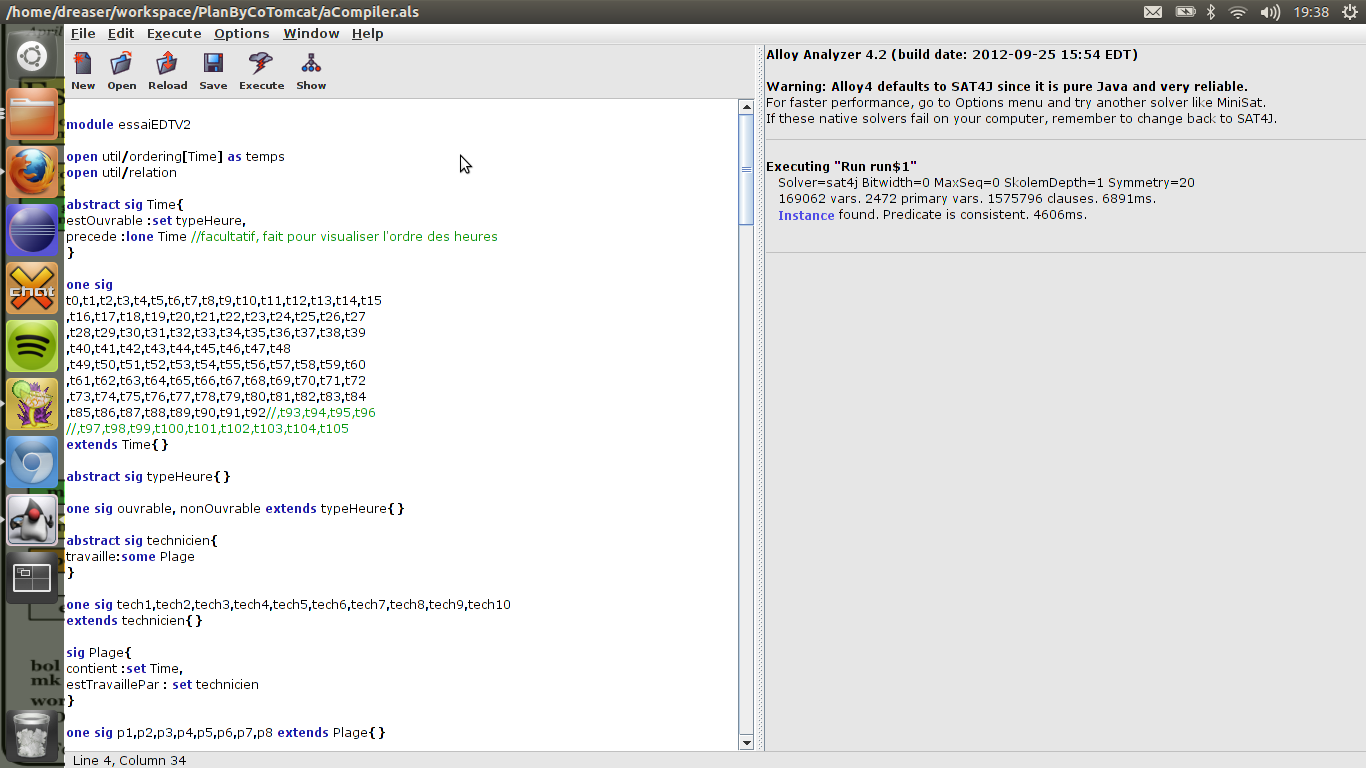
\includegraphics [width=1\textwidth]{images/alloy/GUIalloy.png}
  \end{figure}
\end{center}
\begin{center}
  \begin{figure}[hb]
    \caption{\label{solution} Solution issue du modèle Alloy de mon entreprise}
    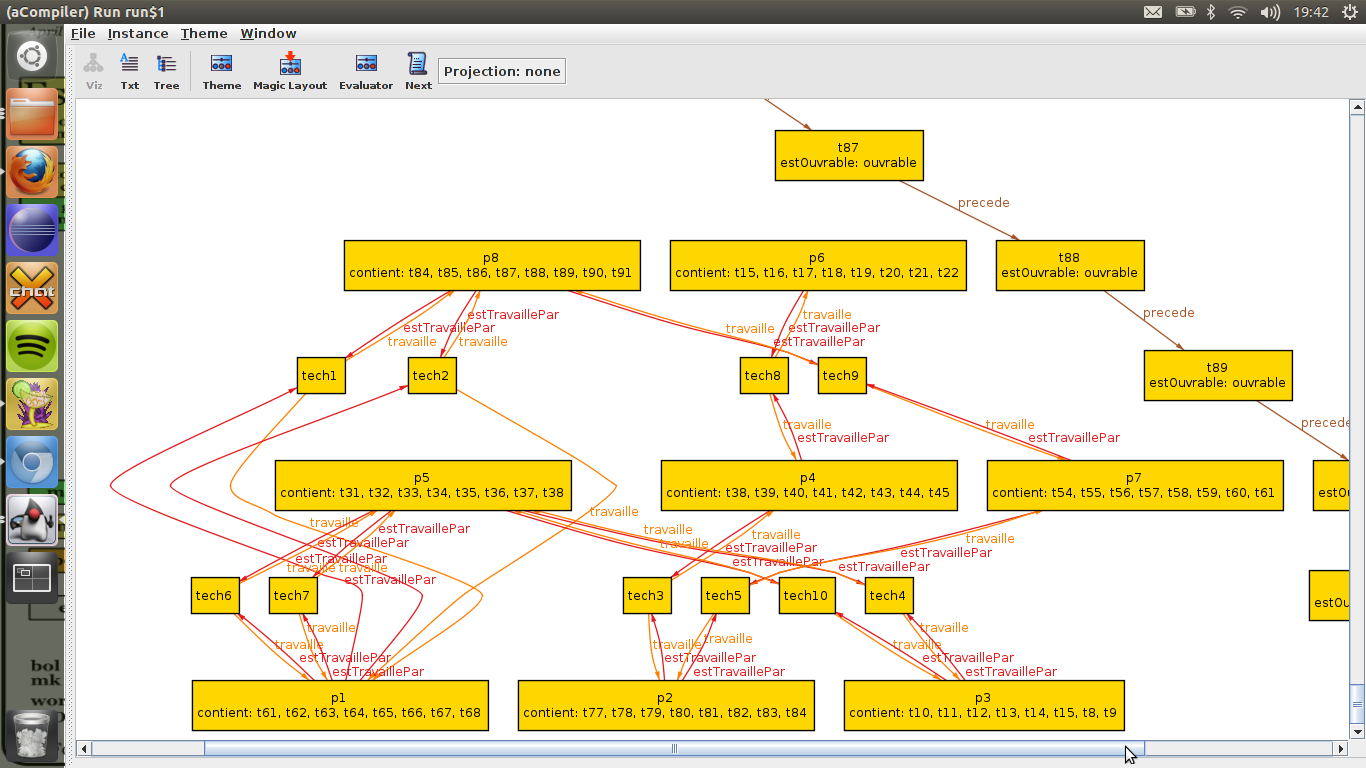
\includegraphics [width=1\textwidth]{images/alloy/solution4j10t.png}
  \end{figure}
\end{center}

La difficulté majeur reposait sur la manière d'exprimer les contraintes. Une contrainte est exprimée de la manière suivante : 
\begin{Verbatim}[frame=single,numbers=left]
//Toutes les plages doivent etre travaillees par au moin un tech
fact{
all p : Plage | some tec : technicien | tec->p in travaille
}
\end{Verbatim}

L'élaboration du modèle Alloy a été la phase la plus difficile de cette mission. Elle a mobilisée une grande partie des mes connaissances mathématiques. C'est finalement avec l'aide de M.\textsc{Bonnot} que j'ai réussi à établir un modèle répondant aux exigences.
Nous avons également choisi de mettre en place un serveur web open-source codé en Java afin de pouvoir le modifier à notre guise. Le fait que le serveur soit codé en Java nous permet également de "piloter" l'\gls{api}\footnote{Une \gls{apidef} est une façade clairement délimitée par laquelle un logiciel offre des services à d'autres logiciels. cf. \url{http://fr.wikipedia.org/wiki/Interface_de_programmation}} via un navigateur internet.
Nous avons d'abord choisi Jetty (une version ancienne car plus facile à modifier), puis j'ai migré vers Tomcat qui s'avère être beaucoup plus flexible et plus simple à manipuler.
Jetty à de nombreux défauts, il ne permettait qu'une réponse en une seul ligne par exemple. De plus chaque requête envoyé par le client devait être gérée manuellement.
\paragraph{}
J'ai également utilisé le \gls{dom}\footnote{Le \gls{domdef} est un standard indépendant de tout langage de programmation permettant la modification de documents XML et HTML. cf. \url{http://fr.wikipedia.org/wiki/Document_Object_Model}} pour générer et interpréter la solution proposée par le compilateur Alloy.
Cette mission n'étant pas achevée, je n'ai pas travaillé l'apparence de l'outil.

\paragraph{}
Parlons maintenant du fonctionnement de l'outil du point de vue du serveur.
Lorsque le serveur reçoit une requête du client, il l'utilise pour recréer le modèle Alloy à partir des différents morceaux stockés dans des fichiers XML. Une fois que le modèle Alloy est reconstitué, il est compilé avec l'\gls{api}. Le résultat est finalement interprété avec le \gls{dom} pour modifier les fichiers HTML qui seront retournés au client.



\subsection{Fonctionnement du point de vue client}%
\paragraph{}
Lorsque l'utilisateur entre l'adresse du site, le serveur renvoi une première page d'accueil avec une première proposition d'emploi du temps "sans contraintes" et un formulaire pour ajouter des contraintes. L'utilisateur peut désormais saisir une première contrainte concernant un technicien en particulier ou une plage horaire en particulier. 
Un nouvelle emploi du temps est généré et retourné au client. Ainsi le client peut modifier à volonté l'emploi du temps.
L'affichage est maintenant beaucoup plus flexible après la migration vers Tomcat étant donnée que Tomcat permet l'utilisation de "Java" dans une page HTML : 
\begin{Verbatim}[frame=single,numbers=left]
<html>
<body>
<table align="center" border="1" summary="" width="80%">
<% 
ArrayList<Jour> attribut = (ArrayList<Jour>)
 request.getAttribute("liste");
for (Jour j : attribut){
	out.println("<tr>");
	out.println("<td>");
	out.println("<b>"+j.getNom()+"</b>");
	out.println("</td>");
	for (PlageHoraire plage : j.getPlagesHoraires()){
		out.println("<td>");
		out.println(plage.getNomPlageHoraire());
		out.println("</td>");
	}
	out.println("</tr>");
}
%>
</table>
</body>
</html>
\end{Verbatim}


Aucune sécurité n'a été mise en place (pour le moment) afin d'éviter que les techniciens ne modifient l'emploi du temps à leur gré sans l'accord du manager.
Toutes les connexions en tant qu'admin ou autres seront gérées en Java directement, donc pas de PHP.
L'archivage des emplois du temps n'est pas non plus opérationnel. Pour l'instant l'emploi du temps est recalculé et stocké à chaque requête  dans un fichier XML. Aucune base de donnée n'est nécessaire.
La seul contrainte inhérente au serveur est qu'il nécessite une machine virtuelle Java.
En effet, du côté client, le site ne nécessite rien d'autre qu'un navigateur supportant le HTML5. 
